% 
% Modelo white-paper 
%
% Marcelo Pereira
%
% 
% e-mail: psnc4ards@gmail.com
%


\documentclass[
	% -- opções da classe memoir --
	article,			% indica que é um artigo acadêmico
	12pt,				% tamanho da fonte
	oneside,			% para impressão apenas no verso. Oposto a twoside
	a4paper,			% tamanho do papel. 
	% -- opções do pacote babel --
	%english,			% idioma adicional para hifenização
	brazil,				% o último idioma é o principal do documento
	english,
	sumario=tradicional
	]{abntex2}


% ---
% PACOTES
% ---

% ---
% Pacotes fundamentais 
% ---
\usepackage{lmodern}			% Usa a fonte Latin Modern
\usepackage[T1]{fontenc}		% Selecao de codigos de fonte.
\usepackage[utf8]{inputenc}		% Codificacao do documento (conversão automática dos acentos)
\usepackage{nomencl} 			% Lista de simbolos
\usepackage{color}				% Controle das cores
\usepackage{graphicx}			% Inclusão de gráficos
\usepackage{microtype} 			% Para melhorias de justificação
\usepackage{float}				% Para ajuste na posição de figuras e tabelas
\usepackage{tikz}
\usepackage{pgf}
\usepackage{adjustbox}
\usepackage{amsmath,amsthm,amsfonts,amssymb}
\definecolor{barblue}{RGB}{153,204,254}
\definecolor{groupblue}{RGB}{51,102,254}
\definecolor{linkred}{RGB}{165,0,33}

\usepackage{amsmath}
\usepackage{tikz}
\usepackage{mathdots}
\usepackage{yhmath}
\usepackage{cancel}
\usepackage{color}
\usepackage{siunitx}
\usepackage{array}
\usepackage{multirow}
\usepackage{amssymb}
\usepackage{gensymb}
\usepackage{tabularx}
\usepackage{booktabs}




% ---
		
% ---
% Pacotes adicionais, usados apenas no âmbito do Modelo Canônico do abnteX2
% ---
\usepackage{lipsum}				% para geração de dummy text
% ---
		
% ---
% Pacotes de citações
% ---
\usepackage[alf]{abntex2cite}	% Citações padrão ABNT
% ---

% ---
% Informações de dados para CAPA e FOLHA DE ROSTO
% ---
\titulo{Reactioon White Paper}
\autor{José Wilker,  \and Jonathas Figueiredo, \and Lucas Tonini}
\local{Brasil}
\data{} 
% ---

% ---
% Alterando o aspecto da cor azul
% ---
\definecolor{blue}{RGB}{41,5,195}
% ---

% ---
% Informações do PDF
% ---
\makeatletter
\hypersetup{
     	%pagebackref=true,
		pdftitle={\@title}, 
		pdfauthor={\@author},
    	pdfsubject={Modelo de artigo científico com abnTeX2},
	    pdfcreator={LaTeX with abnTeX2},
		pdfkeywords={abnt}{latex}{abntex}{abntex2}{artigo científico}, 
		colorlinks=true,       		% false: boxed links; true: colored links
    	linkcolor=blue,          	% color of internal links
    	citecolor=blue,        		% color of links to bibliography
    	filecolor=magenta,      		% color of file links
		urlcolor=blue,
		bookmarksdepth=4
}
\makeatother
% --- 

% ---
% Compila o índice
% ---
\makeindex
% ---

% ---
% Altera as margens padrões
% ---
\setlrmarginsandblock{2cm}{2cm}{*}
\setulmarginsandblock{2cm}{2cm}{*}
\checkandfixthelayout
% ---

% --- 
% Espaçamentos entre linhas e parágrafos 
% --- 

% O tamanho do parágrafo é dado por:
\setlength{\parindent}{.5cm}

% Controle do espaçamento entre um parágrafo e outro:
\setlength{\parskip}{0.2cm}  % tente também \onelineskip

% Espaçamento simples
\SingleSpacing
% ---

% --- 
% Cabeçalho 
% --- 
\makepagestyle{meuestilo}
  \makeoddhead{meuestilo} %%pagina ímpar ou com oneside
     {Reactioon}
     {Vol. 1,  n\textsuperscript{o} 1 (2019)}
     {White-paper 1.2,  page. \thepage}
% ---

% ---
% Margem para resumo, palavras-chave, abstract e keywords
% ---
\def\changemargin#1#2{\list{}{\rightmargin#2\leftmargin#1}\item[]}
\let\endchangemargin=\endlist 
% ----

% ---
% Início do documento
% ---
\begin{document}

% ----------------------------------------------------------
% ELEMENTOS TEXTUAIS
% ----------------------------------------------------------
\textual

% Aplica o cabeçalho em todas as páginas, excetuando-se a primeira
\pagestyle{meuestilo}

% Retira espaço extra obsoleto entre as frases.
\frenchspacing 

% Página de titulo
\maketitle

% Aplica cabeçalho na primeira página
\thispagestyle{meuestilo}
% ---

% -----------------------------------------------------------
% Resumo em português
% -----------------------------------------------------------
\begin{changemargin}{1cm}{1cm} 
 \textbf{Abstract} – The development of Blockchain technology has highlighted an alternative paradigm for financial and non-financial iteration among individuals and organizations. The so-called smart contracts provides a basis for the development of new economic relations in an efficient and safe way. In this white paper we present the Reactioon, a non-possession crypto-asset management platform, which uses artificial intelligence for trading and forecasting. Reactioon aims to become the largest decentralized crypto-assets management network, relying on the symbiosis between in-humans trust and artificial intelligence capacities.
 
 %Use este artigo como modelo para formatar o artigo que você deseja submeter para publicação na Revista Mecatrone.  Inicie o resumo do seu artigo com a palavra “Resumo” em negrito, seguido de um traço.  Os parágrafos de resumo e as palavras-chave (que vem em seguida) devem ter um recuo de 1 cm dos dois lados. Se o artigo não for escrito em inglês, acrescente as versões em inglês do título, resumo e palavras-chaves no final, antes dos minicurrículos dos autores.

 \vspace{\onelineskip}
 
 \noindent
 \textbf{Keywords} – Cripto-assets; Trading; Forecasting; Artificial Intelligence. 
 %artigo científico; formatação; diagramação; estilo 
\end{changemargin}

% ---

%\begin{enumerate}[label=\Alph*]
%\item \textit{Subitem}
%\end{enumerate}

% ----------------------------------------------------------
% Introdução
% ----------------------------------------------------------
\section{Our Vision}
The financial and non-financial utilities that can be structured over blockchain networks are diverse and the quick development of new projects, organizations and contracts based on this technology has created several tokens and altcoins that are currently traded in different exchanges around the world. Most of these projects share the structural basis of the blockchain initiatives: decentralization and security for their users. 

Currently however, the purpose of blockchain technology is partially distorted by centralization mechanisms such as crypto custody enterprises and centralized exchanges. We at Reactioon belive that this scenario is just a transient step towards total decentralization in crypto environment. 

We understand that crypto-currencies and assets traded through smart contracts represent the future of trading in a global economy, we belive that in near future cripto-currencies and contracts will partially replace national cash and government-based contracts around the World. 

Our belief is guided by the Theory of Value and by some historical virtual currencies experiences around the world. Notably some real applications such as WeChat-Pay in China and M-Pesa in Africa reinforce the theory that the market is ready to use virtual crypto-assets making its expansion into all layers of the population  a matter of time and trust.

As part of our contribution to the crypto world we present in this paper a decentralized non-possession crypto-asset management platform aimed to give users the possibility to hold their crypto-assets safe while making profits via limited-access management system, especially by using built-in AI trading system.


\section{Problem Statement}

People who owns crypto-assets usually do so because they believe in the project behind each token or coin, and have attributed a value to it. The price is the result of different in-market interactions and translates people expectations about some good, in this case about crypto-assets.

Because there exists differences in perspective and knowledge about a certain project or coin, the market price of an asset may fluctuate considerably, causing some risk of capital loss as well as some opportunities for short-term gains. The result is that if ones does not properly manage its cripto-portifolio carefully,  it may lead to some capital losses and eventually loss of confidence in the crypto asset itself.

Some centralized custody platforms have come up to fill this gap, they typically offer an alternative opportunity for investors to keep their money safe while making profits from third-party strategies. The most part of these platforms guarantee a fixed return on an initial investment using Bitcoin, Ethereum, or Dollars. The argued method used by them to justify the orign of these returns are usually operations involving trading, arbitrage or buy-and-hold strategies. Unfortunately though, the most part of these platforms are Ponzi schemes aimed to collect money and eventually disappear.  

That is the exactly scenario where Reactioon network take place, we deliver to the crypto community a reliable network platform to handle asset management services with no direct possession, meaning that managers can directly arange someone's portfolio without necessarily keeping the assets. 

% \begin{figure}[H]     % Com o pacote "float", o "[H]" fixa a figura nesse lugar 
%     \centering
%     \includegraphics[width=0.5\textwidth]{figure}
%     \caption{figura}
%     \label{figura}
% \end{figure}



%The interest on this algorithm for the ship problem lies on the fact that it can be used to construct a discrete rudder and thrust control policy, using an approximation for the $Q$ function with relatively few parameters of the Artificial Neural Nework. The counterpart of this method is that it has to be applied together with discrete rudder and propeller actions.


\section{The proposed solution}

In traditional financial market, clients have the option of entrusting custody of their assets to experts managers in stock funds, real estate funds and even trading funds. In this context, the managers have the decision-making power of resource allocation and they seek good investments opportunities aligned with the client suitability level. In this context, fund managers who achieve the greatest success are those who achieve confidence and good historical performance. 

While in traditional market this is the model by which clients are used to have their assets managed, in the crypto-asset market the idea of third-party management of crypto-coins and tokens funds is still recent. Inspired by existing capital management models, we at Reactioon propose a model adapted to the crypto-asset market, based on security, trust and decentralization.

We at Reactioon rely on the following basis for building our crypto-asset management ecosystem:

\begin{itemize}
    \item [1] Management without active crypto possession.
    \item [2] The use of artificial intelligence to perform trade.
    \item [3] Transparency in the relationship between human managers and clients.
    \item [4] Enhance human cognitive abilities using AI.
\end{itemize}
To carry out the Reactioon asset custody network following the basis presented above, we at Reactioon have designed an infrastructure based on the use of trade API tokens issued by exchanges for financial operation. In such way the item 1 of the list above is satisfied, ensuring that Reactioon users have full control of their crypto-assets and are responsible for choosing the organization that holds of their cripto-asset. This is guaranteed since the tokens do not allow any withdraw or external transactions using user funds.

The use of Artificial Intelligence (AI) for trading, as stated in item 2, is a service provided by Reactioon network that allows users to make profits by taking advantage of the volatility of a given criptocurrency pair. By using market forecasting, a preprogrammed artificial intelligence algorithm performs automatic trade into users exchanges accounts and even provide signals for hand-operated trading. In order to access the trading services customers have to using Reactioon (RTN) currency, issued during the project ICO.

As part of our strategy of decentralization and transparency (item 3), the user of Reactioon network can choose which Exchanges to trust their coins custody,  ensuring that each user is free to choose which institution to trust the security of their coins. The Reactioon development team is working every day to increase the number of supported Exchange, our goal is to include decentralized Exchange as a way to strengthen the project's decentralization philosophy. More details about the supported Exchanges can be found in the Roadmap section.

In addition to the use of robots for trading management, we at Reactioon propose in our platform a model in which users with the status of Managers will be able to create their own investment funds for managing funds of investing users. In this case, investing users can choose in which fund / manager to invest based on trust and  historical data performance. In our design the fund manager receives the payment for his services through the Reactioon token (RTN) that can be further resold on the market.

We at Reactioon see a great potential in human-management crypto-asset funds, we understand that in the medium-term many of the securities currently traded on the stock market will be traded through smart contracts,  making the Reactioon environment a possible structure where these trades will take place. 

In this context, we plan to provide data to support human managers through technical and fundamental analysis using artificial intelligence technology. The data may include portfolio recommendations and probabilistic analyzes based on asset characteristics, historical analysis and economic context. By helping managers in decision making, we follow the global trend for increasing human cognitive performance aided by AI technology as stated in item 4.

Figure 1 presents a simplified diagram of the Reactioon Network. The network is composed by two different types of nodes, AI-based nodes and Human-based nodes. Nodes are structures containing strategic decision algorithms and are the interface by which clients can consign their asset management to a third-party entity (AI or human-manager). 

A Client who prefers to trust his assets to an AI manager (Client X) may provide his API token issued by the Exchange in which he keeps the funds. In this case, to contract an AI trading strategy service client X must choose some settings such as risk level currency pair, etc, before start the trade contract. Finally, in order to run the AI-trading management contract, client X has to pay a fixed amount of Reactioon token (RTN) for a delimited period of time (i.e 30 days). While the contract is running, the clients funds at Exchange X will be traded directly by the node algorithm. The node owner will recieve the respective amount of RTN token paid by client X for each day of trading service provided.

On the same way, a client who prefers to trust his assets to a Human manager (Client Y) may provide his API token issued by the Exchange in which he keeps the funds. Once client Y has chosen the fund manager and the type of portfolio (high, medium or low risk) he must pay a certain amount of RTN token start the management contract. The human manager will manually send the purchase and sale orders of a given asset directly to the exchange of client Y. The manager will receive the RTN tokens as his strategy is being periodically applied.


\begin{figure}[H]
    \centering
    \makebox[\textwidth]{


\tikzset{every picture/.style={line width=0.75pt}} %set default line width to 0.75pt        

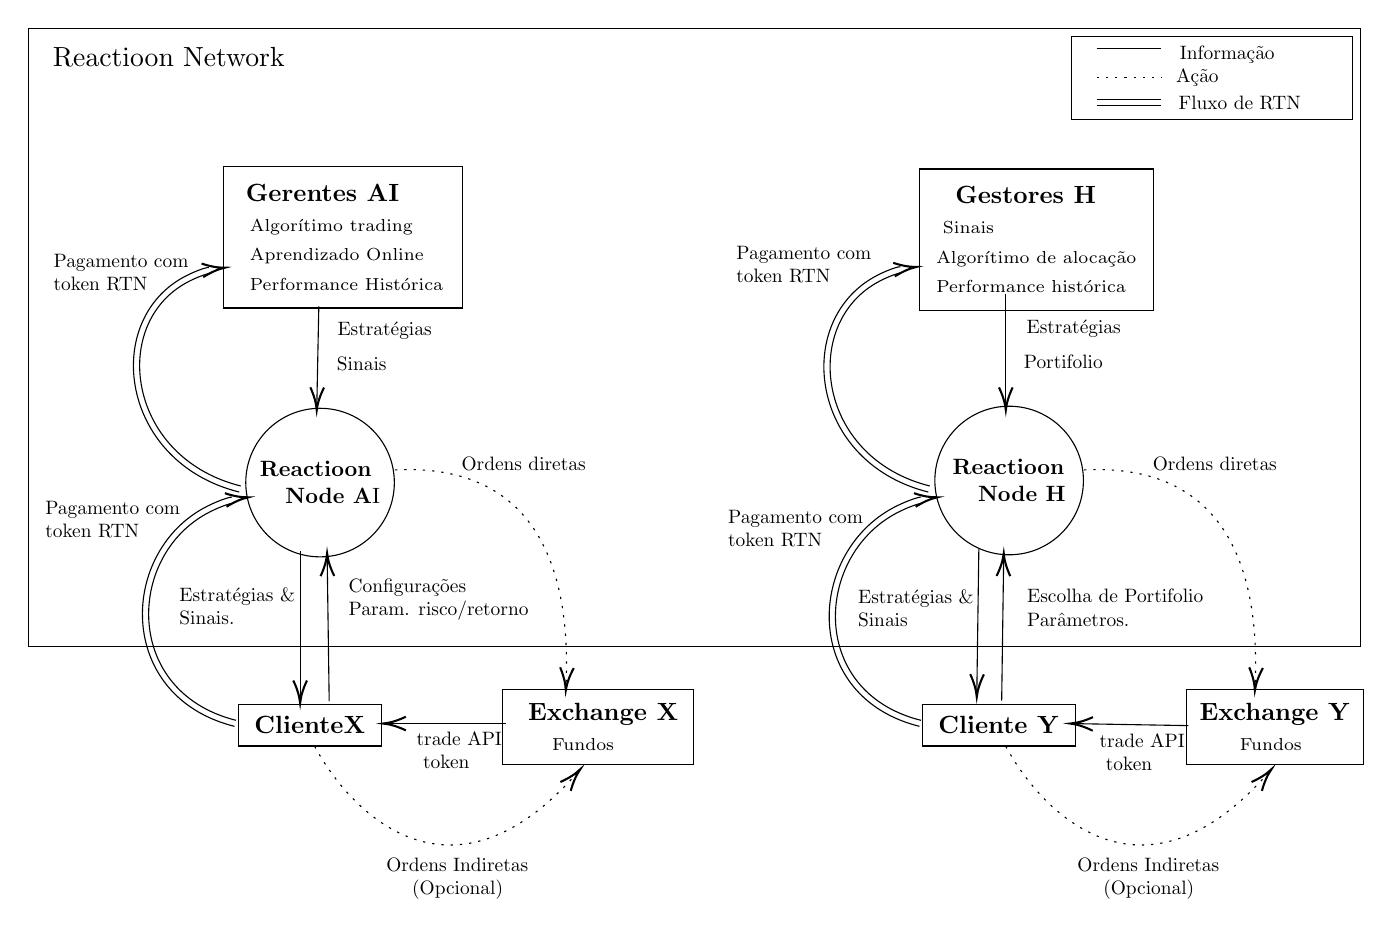
\begin{tikzpicture}[x=0.75pt,y=0.75pt,yscale=-1,xscale=1]
%uncomment if require: \path (0,464.1999969482422); %set diagram left start at 0, and has height of 464.1999969482422

%Shape: Rectangle [id:dp839607811925092] 
\draw   (16.3,16.2) -- (658.3,16.2) -- (658.3,314.2) -- (16.3,314.2) -- cycle ;
%Straight Lines [id:da3953078356379509] 
\draw    (156.3,150.2) -- (155.34,198.2) ;
\draw [shift={(155.3,200.2)}, rotate = 271.15] [color={rgb, 255:red, 0; green, 0; blue, 0 }  ][line width=0.75]    (10.93,-3.29) .. controls (6.95,-1.4) and (3.31,-0.3) .. (0,0) .. controls (3.31,0.3) and (6.95,1.4) .. (10.93,3.29)   ;

%Straight Lines [id:da5714023605084257] 
\draw    (246.3,351.2) -- (189.3,351.2) ;
\draw [shift={(187.3,351.2)}, rotate = 360] [color={rgb, 255:red, 0; green, 0; blue, 0 }  ][line width=0.75]    (10.93,-3.29) .. controls (6.95,-1.4) and (3.31,-0.3) .. (0,0) .. controls (3.31,0.3) and (6.95,1.4) .. (10.93,3.29)   ;

%Straight Lines [id:da41026468235715097] 
\draw    (161.3,340.4) -- (160.33,271.2) ;
\draw [shift={(160.3,269.2)}, rotate = 449.2] [color={rgb, 255:red, 0; green, 0; blue, 0 }  ][line width=0.75]    (10.93,-3.29) .. controls (6.95,-1.4) and (3.31,-0.3) .. (0,0) .. controls (3.31,0.3) and (6.95,1.4) .. (10.93,3.29)   ;

%Curve Lines [id:da9188372161085148] 
\draw  [dash pattern={on 0.84pt off 2.51pt}]  (193,229) .. controls (247.03,226.21) and (278.98,257.88) .. (275.36,334.05) ;
\draw [shift={(275.3,335.2)}, rotate = 272.97] [color={rgb, 255:red, 0; green, 0; blue, 0 }  ][line width=0.75]    (10.93,-3.29) .. controls (6.95,-1.4) and (3.31,-0.3) .. (0,0) .. controls (3.31,0.3) and (6.95,1.4) .. (10.93,3.29)   ;

%Curve Lines [id:da6611499345431215] 
\draw    (115.68,352.55) .. controls (92.15,346.66) and (78.57,331.56) .. (73.55,314.31) .. controls (72.05,309.15) and (71.32,303.8) .. (71.32,298.44) .. controls (71.32,298.19) and (71.32,297.93) .. (71.32,297.68) .. controls (71.58,277.85) and (81.85,258.04) .. (100.37,247.66) .. controls (106.22,244.39) and (112.89,242.05) .. (114.47,242.1)(116.41,349.64) .. controls (94.14,344.07) and (81.19,329.83) .. (76.43,313.47) .. controls (75.01,308.58) and (74.32,303.52) .. (74.32,298.44) .. controls (74.32,298.2) and (74.32,297.96) .. (74.32,297.72) .. controls (74.56,278.93) and (84.27,260.12) .. (101.84,250.28) .. controls (107.38,247.17) and (113.71,244.96) .. (114.91,245.09) ;
\draw [shift={(122.3,242.2)}, rotate = 533.23] [color={rgb, 255:red, 0; green, 0; blue, 0 }  ][line width=0.75]    (10.93,-3.29) .. controls (6.95,-1.4) and (3.31,-0.3) .. (0,0) .. controls (3.31,0.3) and (6.95,1.4) .. (10.93,3.29)   ;

%Curve Lines [id:da6558944188118099] 
\draw    (117.94,239.66) .. controls (91.22,232.98) and (75.05,214.75) .. (69.33,195.07) .. controls (68.48,192.12) and (67.85,189.14) .. (67.47,186.16) .. controls (67.14,183.68) and (66.98,181.21) .. (66.98,178.76) .. controls (66.98,161.73) and (74.72,145.63) .. (90.09,136.73) .. controls (95.48,133.61) and (101.81,131.38) .. (103.3,131.45)(118.66,236.74) .. controls (93.17,230.37) and (77.68,213.04) .. (72.22,194.23) .. controls (71.4,191.43) and (70.81,188.6) .. (70.44,185.77) .. controls (70.14,183.43) and (69.98,181.08) .. (69.98,178.76) .. controls (69.98,162.8) and (77.17,147.68) .. (91.6,139.33) .. controls (96.68,136.39) and (102.66,134.28) .. (103.68,134.45) ;
\draw [shift={(111.06,131.56)}, rotate = 533.23] [color={rgb, 255:red, 0; green, 0; blue, 0 }  ][line width=0.75]    (10.93,-3.29) .. controls (6.95,-1.4) and (3.31,-0.3) .. (0,0) .. controls (3.31,0.3) and (6.95,1.4) .. (10.93,3.29)   ;

%Curve Lines [id:da7197337789763143] 
\draw  [dash pattern={on 0.84pt off 2.51pt}]  (154.3,362.2) .. controls (173.2,397.02) and (221.81,442.74) .. (281.4,374.24) ;
\draw [shift={(282.3,373.2)}, rotate = 490.6] [color={rgb, 255:red, 0; green, 0; blue, 0 }  ][line width=0.75]    (10.93,-3.29) .. controls (6.95,-1.4) and (3.31,-0.3) .. (0,0) .. controls (3.31,0.3) and (6.95,1.4) .. (10.93,3.29)   ;

%Straight Lines [id:da7501707624311069] 
\draw    (487.3,144.2) -- (487.3,198.2) ;
\draw [shift={(487.3,200.2)}, rotate = 270] [color={rgb, 255:red, 0; green, 0; blue, 0 }  ][line width=0.75]    (10.93,-3.29) .. controls (6.95,-1.4) and (3.31,-0.3) .. (0,0) .. controls (3.31,0.3) and (6.95,1.4) .. (10.93,3.29)   ;

%Straight Lines [id:da11297405436688912] 
\draw    (575.3,352.2) -- (520.3,351.24) ;
\draw [shift={(518.3,351.2)}, rotate = 361.01] [color={rgb, 255:red, 0; green, 0; blue, 0 }  ][line width=0.75]    (10.93,-3.29) .. controls (6.95,-1.4) and (3.31,-0.3) .. (0,0) .. controls (3.31,0.3) and (6.95,1.4) .. (10.93,3.29)   ;

%Straight Lines [id:da9530469398494208] 
\draw    (485.3,340.2) -- (486.27,271.2) ;
\draw [shift={(486.3,269.2)}, rotate = 450.81] [color={rgb, 255:red, 0; green, 0; blue, 0 }  ][line width=0.75]    (10.93,-3.29) .. controls (6.95,-1.4) and (3.31,-0.3) .. (0,0) .. controls (3.31,0.3) and (6.95,1.4) .. (10.93,3.29)   ;

%Curve Lines [id:da6669727888364709] 
\draw  [dash pattern={on 0.84pt off 2.51pt}]  (525,229) .. controls (579.03,226.21) and (610.98,257.88) .. (607.36,334.05) ;
\draw [shift={(607.3,335.2)}, rotate = 272.97] [color={rgb, 255:red, 0; green, 0; blue, 0 }  ][line width=0.75]    (10.93,-3.29) .. controls (6.95,-1.4) and (3.31,-0.3) .. (0,0) .. controls (3.31,0.3) and (6.95,1.4) .. (10.93,3.29)   ;

%Curve Lines [id:da6929077991045711] 
\draw    (445.68,352.55) .. controls (422.54,346.76) and (409.27,332.05) .. (404.37,315.16) .. controls (402.91,310.12) and (402.2,304.87) .. (402.2,299.6) .. controls (402.2,298.95) and (402.21,298.3) .. (402.23,297.65) .. controls (402.9,277.57) and (413.86,257.51) .. (433.02,247.25) .. controls (438.74,244.19) and (445.19,242) .. (446.5,242.09)(446.41,349.64) .. controls (424.53,344.17) and (411.89,330.33) .. (407.26,314.33) .. controls (405.87,309.55) and (405.2,304.59) .. (405.2,299.6) .. controls (405.2,298.98) and (405.21,298.36) .. (405.23,297.75) .. controls (405.86,278.7) and (416.25,259.64) .. (434.43,249.9) .. controls (439.87,246.99) and (445.99,244.92) .. (446.94,245.08) ;
\draw [shift={(454.3,242.2)}, rotate = 533.23] [color={rgb, 255:red, 0; green, 0; blue, 0 }  ][line width=0.75]    (10.93,-3.29) .. controls (6.95,-1.4) and (3.31,-0.3) .. (0,0) .. controls (3.31,0.3) and (6.95,1.4) .. (10.93,3.29)   ;

%Curve Lines [id:da46112590181388846] 
\draw    (449.94,239.66) .. controls (423.51,233.05) and (407.61,215.09) .. (401.97,195.59) .. controls (401.05,192.4) and (400.4,189.18) .. (400.03,185.95) .. controls (399.77,183.73) and (399.64,181.5) .. (399.64,179.29) .. controls (399.64,162) and (407.53,145.57) .. (423.1,136.49) .. controls (428.56,133.31) and (434.97,131.03) .. (436.48,131.11)(450.66,236.74) .. controls (425.47,230.45) and (410.24,213.37) .. (404.85,194.75) .. controls (403.98,191.73) and (403.36,188.67) .. (403.01,185.61) .. controls (402.76,183.5) and (402.64,181.39) .. (402.64,179.29) .. controls (402.64,163.07) and (409.98,147.61) .. (424.62,139.09) .. controls (429.77,136.08) and (435.82,133.94) .. (436.95,134.08) ;
\draw [shift={(444.3,131.2)}, rotate = 533.23] [color={rgb, 255:red, 0; green, 0; blue, 0 }  ][line width=0.75]    (10.93,-3.29) .. controls (6.95,-1.4) and (3.31,-0.3) .. (0,0) .. controls (3.31,0.3) and (6.95,1.4) .. (10.93,3.29)   ;

%Curve Lines [id:da8354818907327548] 
\draw  [dash pattern={on 0.84pt off 2.51pt}]  (487.3,362.2) .. controls (506.2,397.02) and (554.81,442.74) .. (614.4,374.24) ;
\draw [shift={(615.3,373.2)}, rotate = 490.6] [color={rgb, 255:red, 0; green, 0; blue, 0 }  ][line width=0.75]    (10.93,-3.29) .. controls (6.95,-1.4) and (3.31,-0.3) .. (0,0) .. controls (3.31,0.3) and (6.95,1.4) .. (10.93,3.29)   ;

%Straight Lines [id:da8770926699692774] 
\draw    (147.3,268.2) -- (147.3,339.4) ;
\draw [shift={(147.3,341.4)}, rotate = 270] [color={rgb, 255:red, 0; green, 0; blue, 0 }  ][line width=0.75]    (10.93,-3.29) .. controls (6.95,-1.4) and (3.31,-0.3) .. (0,0) .. controls (3.31,0.3) and (6.95,1.4) .. (10.93,3.29)   ;

%Straight Lines [id:da36937072037759555] 
\draw    (474.3,267.2) -- (473.33,336.4) ;
\draw [shift={(473.3,338.4)}, rotate = 270.8] [color={rgb, 255:red, 0; green, 0; blue, 0 }  ][line width=0.75]    (10.93,-3.29) .. controls (6.95,-1.4) and (3.31,-0.3) .. (0,0) .. controls (3.31,0.3) and (6.95,1.4) .. (10.93,3.29)   ;

%Shape: Rectangle [id:dp03825033305531944] 
\draw   (518.9,20) -- (654.3,20) -- (654.3,60) -- (518.9,60) -- cycle ;
%Straight Lines [id:da5606203321141707] 
\draw    (531,26) -- (562.3,26) ;


%Straight Lines [id:da21375108102279738] 
\draw  [dash pattern={on 0.84pt off 2.51pt}]  (531,40) -- (562.3,40) ;


%Straight Lines [id:da15988012489637837] 
\draw    (531,50.5) -- (562.3,50.5)(531,53.5) -- (562.3,53.5) ;



% Text Node
\draw    (245,335) -- (337,335) -- (337,371) -- (245,371) -- cycle  ;
\draw (291,353) node [scale=0.9] [align=left] {\textbf{ Exchange X }\\{\scriptsize  \ \ \ \ \ Fundos}};
% Text Node
\draw    (117.5,342) -- (186.5,342) -- (186.5,362) -- (117.5,362) -- cycle  ;
\draw (152,352) node [scale=0.9] [align=left] {\textbf{ ClienteX }};
% Text Node
\draw    (110.5,83) -- (225.5,83) -- (225.5,151) -- (110.5,151) -- cycle  ;
\draw (168,117) node [scale=0.9] [align=left] {\textbf{ Gerentes AI}\\{\scriptsize  \ \ Algorítimo trading}\\{\scriptsize  \ \ Aprendizado Online \ }\\{\scriptsize  \ \ Performance Histórica \ }};
% Text Node
\draw    (156.9, 235.1) circle [x radius= 35.79, y radius= 35.79]   ;
\draw (156.9,235.1) node [scale=0.8] [align=left] {\textbf{Reactioon}\\\textbf{ \ \ Node A}I};
% Text Node
\draw (84,30) node  [align=left] {Reactioon Network};
% Text Node
\draw (224,364) node [scale=0.7] [align=left] {trade API \\ \ token};
% Text Node
\draw (188,162) node [scale=0.7] [align=left] {Estratégias};
% Text Node
\draw (177,178) node [scale=0.7] [align=left] {Sinais};
% Text Node
\draw (214,296) node [scale=0.7] [align=left] {Configurações\\Param. risco/retorno\\};
% Text Node
\draw (61,134) node [scale=0.7] [align=left] {Pagamento com\\ token RTN};
% Text Node
\draw (255,226) node [scale=0.7] [align=left] {Ordens diretas};
% Text Node
\draw (223,426) node [scale=0.7] [align=left] {Ordens Indiretas\\ \ \ \ \ (Opcional)};
% Text Node
\draw    (574.5,335) -- (659.5,335) -- (659.5,371) -- (574.5,371) -- cycle  ;
\draw (617,353) node [scale=0.9] [align=left] {\textbf{Exchange Y}\\{\scriptsize  \ \ \ \ \ \ Fundos}};
% Text Node
\draw    (447,342) -- (521,342) -- (521,362) -- (447,362) -- cycle  ;
\draw (484,352) node [scale=0.9] [align=left] {\textbf{ Cliente Y }};
% Text Node
\draw    (445.5,84) -- (558.5,84) -- (558.5,152) -- (445.5,152) -- cycle  ;
\draw (502,118) node [scale=0.9] [align=left] {\textbf{ \ Gestores H}\\{\scriptsize  \ Sinais}\\ {\scriptsize Algorítimo de alocação \ }\\{\scriptsize  Performance histórica }};
% Text Node
\draw    (488.9, 234.1) circle [x radius= 35.79, y radius= 35.79]   ;
\draw (488.9,234.1) node [scale=0.8] [align=left] {\textbf{Reactioon}\\\textbf{ \ \ Node H}};
% Text Node
\draw (540,301) node [scale=0.7] [align=left] {Escolha de Portifolio\\Parâmetros.\\};
% Text Node
\draw (588,226) node [scale=0.7] [align=left] {Ordens diretas};
% Text Node
\draw (117,306) node [scale=0.7] [align=left] {Estratégias \&\\Sinais.\\\\};
% Text Node
\draw (444,307) node [scale=0.7] [align=left] {Estratégias \&\\Sinais\\\\};
% Text Node
\draw (579.6,40) node [scale=0.7] [align=left] {Ação};
% Text Node
\draw (594,29) node [scale=0.7] [align=left] {Informação};
% Text Node
\draw (600,52) node [scale=0.7] [align=left] {Fluxo de RTN};
% Text Node
\draw (553,365) node [scale=0.7] [align=left] {trade API \\ \ token};
% Text Node
\draw (390,130) node [scale=0.7] [align=left] {Pagamento com\\ token RTN};
% Text Node
\draw (520,161) node [scale=0.7] [align=left] {Estratégias};
% Text Node
\draw (515,177) node [scale=0.7] [align=left] {Portifolio};
% Text Node
\draw (57,253) node [scale=0.7] [align=left] {Pagamento com\\ token RTN};
% Text Node
\draw (386,257) node [scale=0.7] [align=left] {Pagamento com\\ token RTN};
% Text Node
\draw (556,426) node [scale=0.7] [align=left] {Ordens Indiretas\\ \ \ \ \ (Opcional)};


\end{tikzpicture}
}
\caption{Reactioon network diagram}
\end{figure}

In both forms of management contract the client can choose not to provide the API key of his exchange, in this case however the client have to perform the trades by hand based on the real-time trading signals provided by the Reactioon nodes. This option is not recommended for AI trading strategies and short-term strategies managed by humans.

\section{Roadmap}
\subsection{Development steps}
This section presents the Roadmap of Reactioon project, describing each development step and our main goals. Figure 2 depict all planned steps.

STEP 0 is the project Initial Coin Offer (ICO). During this step RTN tokens will be issued to investors who are aligned with our ideas interested in our project. We see 3 different types of investor:
\begin{itemize}
    \item Level-0 refers to  investor looking for gains with buy and hold strategy using RTN tokens. 
    \item Level-1 refers to investors aiming to use platform as clients of our management services. 
    \item Level 3 refers to investors planning to buy and run their own nodes in near future. 
\end{itemize}

STEP 1 is the project Proof of concept. This step is planned to run in parallel with the project ICO as a way to endorse the project trust and reputation. During this step a list of Exchanges are planned to be included in the project trade API system.





\begin{figure}[H]
    \centering
    \makebox[\textwidth]{


\tikzset{every picture/.style={line width=0.75pt}} %set default line width to 0.75pt        

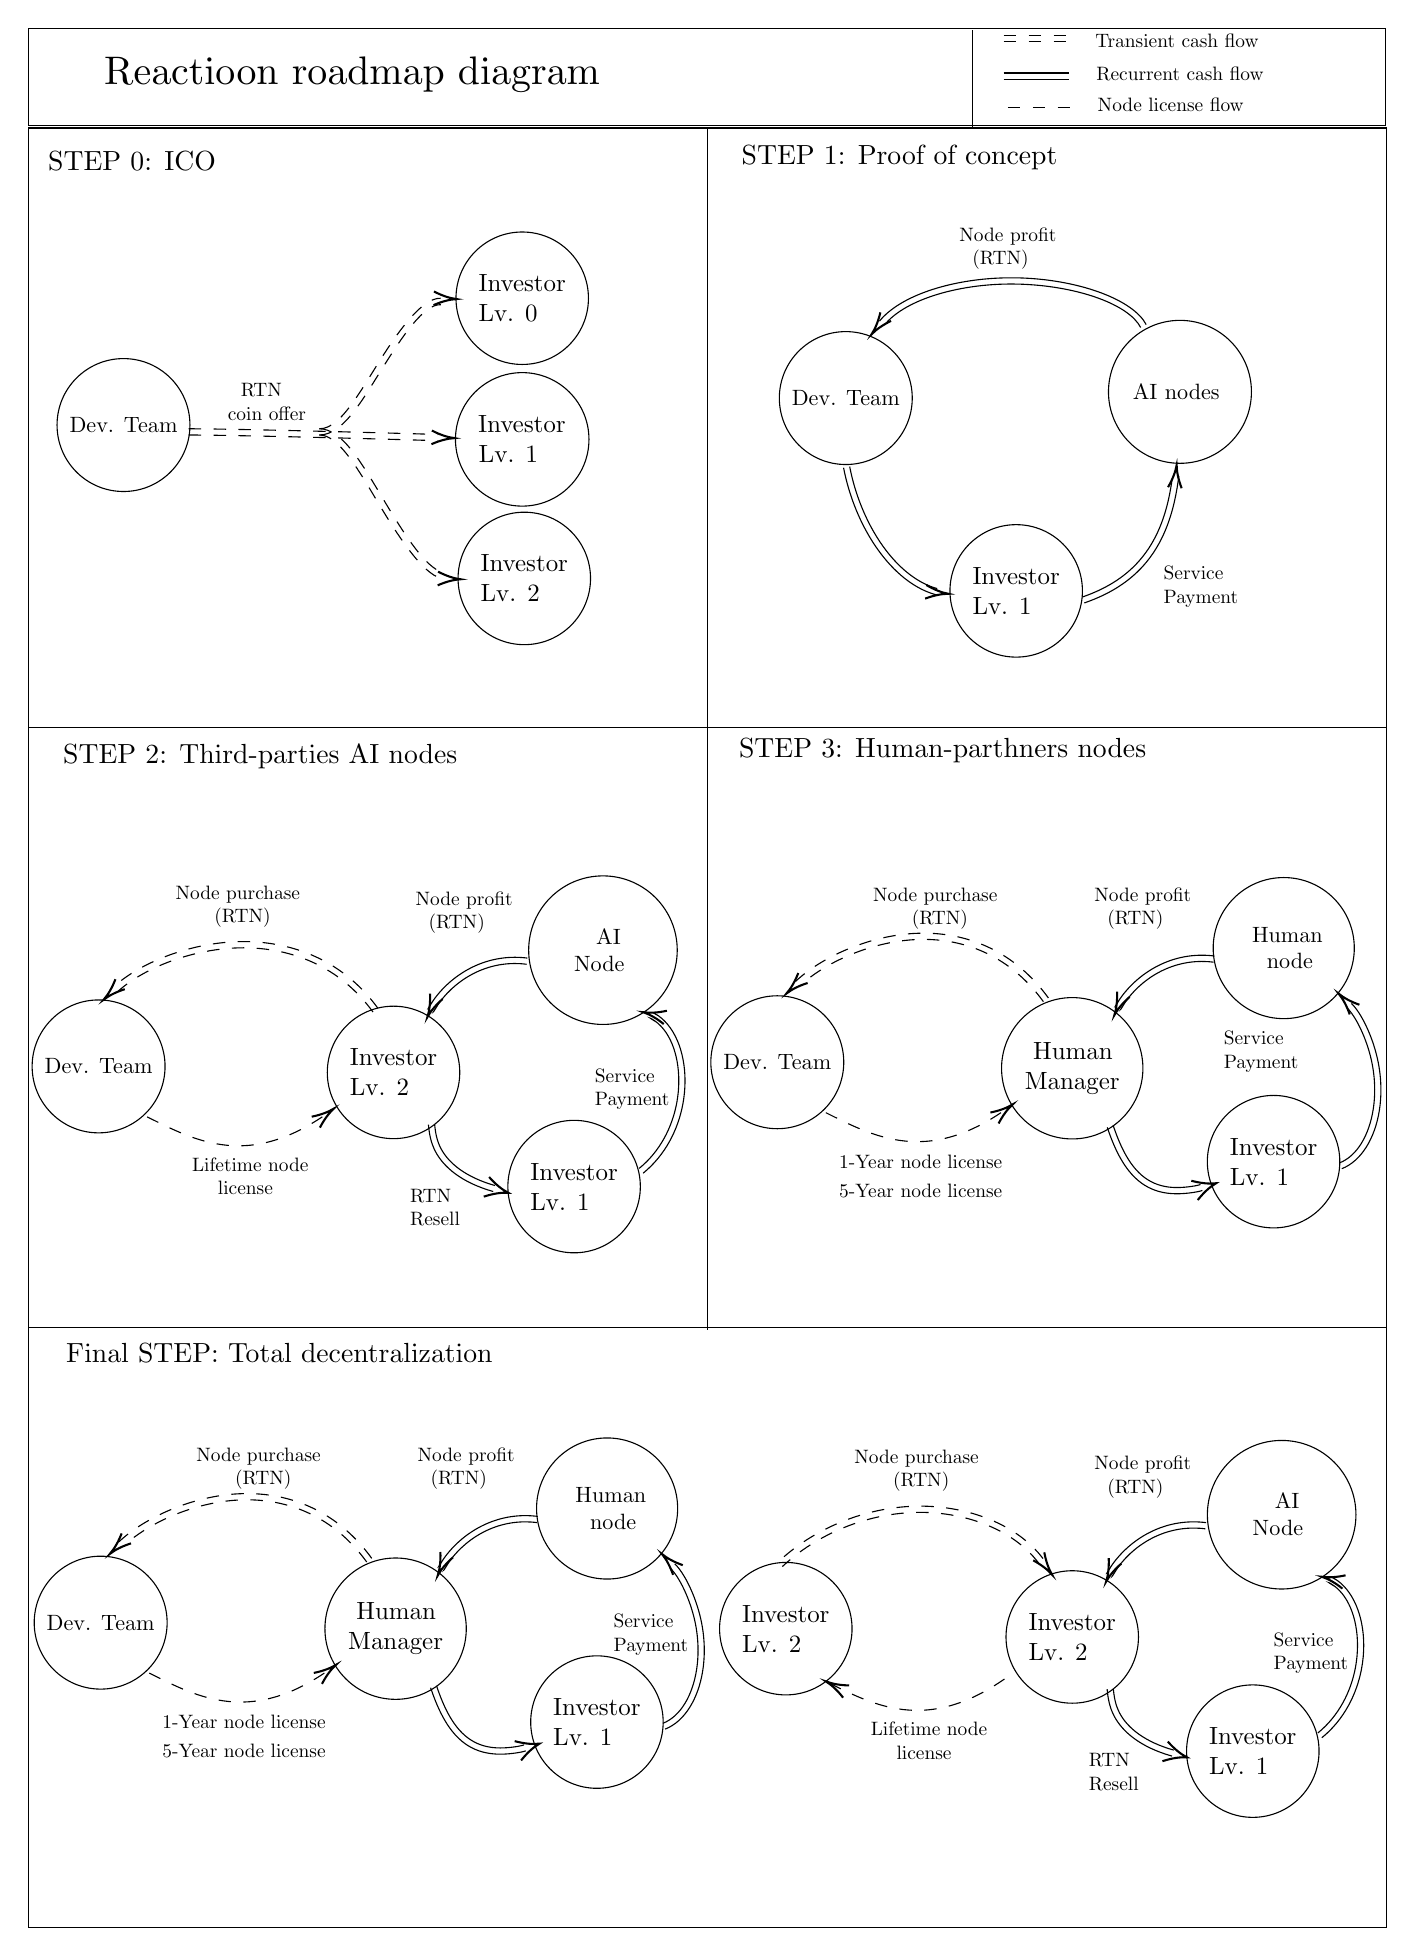
\begin{tikzpicture}[x=0.75pt,y=0.75pt,yscale=-1,xscale=1]
%uncomment if require: \path (0,979.6000061035156); %set diagram left start at 0, and has height of 979.6000061035156

%Curve Lines [id:da05976634933651925] 
\draw    (396.77,250.11) .. controls (401.92,276.72) and (417.5,301.22) .. (436.51,308.13) .. controls (438.57,308.87) and (440.67,309.41) .. (436.98,308.29)(393.83,250.69) .. controls (399.21,278.49) and (415.72,303.77) .. (435.49,310.95) .. controls (437.74,311.76) and (440.04,312.35) .. (436.54,311.31) ;
\draw [shift={(444.3,311.4)}, rotate = 184.97] [color={rgb, 255:red, 0; green, 0; blue, 0 }  ][line width=0.75]    (10.93,-3.29) .. controls (6.95,-1.4) and (3.31,-0.3) .. (0,0) .. controls (3.31,0.3) and (6.95,1.4) .. (10.93,3.29)   ;

%Curve Lines [id:da6305771665750117] 
\draw    (508.81,312.98) .. controls (530.84,305.36) and (545.51,291.1) .. (550.94,263.26) .. controls (551.69,259.42) and (552.27,255.33) .. (551.99,256.88)(509.79,315.82) .. controls (532.83,307.84) and (548.21,292.97) .. (553.89,263.83) .. controls (554.66,259.9) and (555.24,255.71) .. (554.98,257.17) ;
\draw [shift={(554.3,249.4)}, rotate = 454.51] [color={rgb, 255:red, 0; green, 0; blue, 0 }  ][line width=0.75]    (10.93,-3.29) .. controls (6.95,-1.4) and (3.31,-0.3) .. (0,0) .. controls (3.31,0.3) and (6.95,1.4) .. (10.93,3.29)   ;

%Curve Lines [id:da2780992376736433] 
\draw    (536.97,183.09) .. controls (531.13,171.91) and (506.97,163.46) .. (480.65,162.29) .. controls (478.64,162.2) and (476.6,162.16) .. (474.57,162.16) .. controls (472.28,162.16) and (469.98,162.21) .. (467.68,162.33) .. controls (445.29,163.49) and (422.84,170.39) .. (413.48,181.92)(539.63,181.71) .. controls (533.53,170.01) and (508.64,160.53) .. (480.78,159.29) .. controls (478.72,159.2) and (476.65,159.16) .. (474.57,159.16) .. controls (472.23,159.16) and (469.88,159.22) .. (467.53,159.34) .. controls (444.26,160.54) and (421.05,167.87) .. (411.11,180.04) ;
\draw [shift={(407.3,186.4)}, rotate = 308.65999999999997] [color={rgb, 255:red, 0; green, 0; blue, 0 }  ][line width=0.75]    (10.93,-3.29) .. controls (6.95,-1.4) and (3.31,-0.3) .. (0,0) .. controls (3.31,0.3) and (6.95,1.4) .. (10.93,3.29)   ;

%Curve Lines [id:da09682931505407599] 
\draw    (295.35,588.24) .. controls (305.49,579.98) and (311.3,568.29) .. (313.47,556.61) .. controls (314.12,553.06) and (314.44,549.5) .. (314.44,546.05) .. controls (314.44,533.02) and (309.94,521.23) .. (301.62,516.34) .. controls (300.63,515.76) and (299.6,515.28) .. (303.74,517.8)(297.25,590.56) .. controls (307.96,581.84) and (314.13,569.5) .. (316.42,557.15) .. controls (317.11,553.42) and (317.44,549.68) .. (317.44,546.05) .. controls (317.44,531.72) and (312.19,519.07) .. (303.14,513.75) .. controls (301.98,513.07) and (300.76,512.5) .. (304.78,514.82) ;
\draw [shift={(297.3,513)}, rotate = 373.21000000000004] [color={rgb, 255:red, 0; green, 0; blue, 0 }  ][line width=0.75]    (10.93,-3.29) .. controls (6.95,-1.4) and (3.31,-0.3) .. (0,0) .. controls (3.31,0.3) and (6.95,1.4) .. (10.93,3.29)   ;

%Straight Lines [id:da7893540143315829] 
\draw    (328.22,87) -- (328.22,666.2) ;


%Curve Lines [id:da1024768683684969] 
\draw    (225.02,599.37) .. controls (209.68,595.06) and (201.11,587.53) .. (197.2,580.12) .. controls (194.86,575.68) and (194.19,571.25) .. (193.81,567.14)(225.91,596.51) .. controls (211.81,592.55) and (203.54,585.7) .. (199.86,578.72) .. controls (197.72,574.66) and (197.14,570.61) .. (196.79,566.86) ;

\draw [shift={(232.3,600)}, rotate = 195.26] [color={rgb, 255:red, 0; green, 0; blue, 0 }  ][line width=0.75]    (10.93,-4.9) .. controls (6.95,-2.3) and (3.31,-0.67) .. (0,0) .. controls (3.31,0.67) and (6.95,2.3) .. (10.93,4.9)   ;
%Curve Lines [id:da669725253916299] 
\draw  [dash pattern={on 4.5pt off 4.5pt}]  (167.09,512.88) .. controls (151.26,491.1) and (128.15,481.96) .. (104.77,481.96) .. controls (103.86,481.96) and (102.94,481.98) .. (102.02,482) .. controls (78.89,482.71) and (55.75,492.2) .. (43.67,503.46)(169.51,511.12) .. controls (153.07,488.49) and (129.07,478.96) .. (104.77,478.96) .. controls (103.83,478.96) and (102.88,478.98) .. (101.93,479) .. controls (78.08,479.73) and (54.24,489.52) .. (41.78,501.13) ;
\draw [shift={(37.3,507)}, rotate = 316.74] [color={rgb, 255:red, 0; green, 0; blue, 0 }  ][line width=0.75]    (10.93,-3.29) .. controls (6.95,-1.4) and (3.31,-0.3) .. (0,0) .. controls (3.31,0.3) and (6.95,1.4) .. (10.93,3.29)   ;

%Curve Lines [id:da8285498578095596] 
\draw    (195.99,507.55) .. controls (193.21,512.09) and (193.61,511.35) .. (194.04,510.61) .. controls (201.02,498.57) and (215.98,486.53) .. (235.47,486.53) .. controls (237.43,486.53) and (239.44,486.66) .. (241.49,486.91)(198.71,508.9) .. controls (195.87,513.49) and (196.24,512.8) .. (196.63,512.12) .. controls (203.18,500.83) and (217.2,489.53) .. (235.47,489.53) .. controls (237.31,489.53) and (239.19,489.65) .. (241.11,489.89) ;

\draw [shift={(193.3,515.4)}, rotate = 293.2] [color={rgb, 255:red, 0; green, 0; blue, 0 }  ][line width=0.75]    (10.93,-3.29) .. controls (6.95,-1.4) and (3.31,-0.3) .. (0,0) .. controls (3.31,0.3) and (6.95,1.4) .. (10.93,3.29)   ;
%Curve Lines [id:da692172908683615] 
\draw  [dash pattern={on 4.5pt off 4.5pt}]  (58.3,563.4) .. controls (82.06,575.28) and (107.78,589.12) .. (147.1,560.29) ;
\draw [shift={(148.3,559.4)}, rotate = 503.13] [color={rgb, 255:red, 0; green, 0; blue, 0 }  ][line width=0.75]    (10.93,-3.29) .. controls (6.95,-1.4) and (3.31,-0.3) .. (0,0) .. controls (3.31,0.3) and (6.95,1.4) .. (10.93,3.29)   ;

%Shape: Rectangle [id:dp40281470565409405] 
\draw   (1,87) -- (655.3,87) -- (655.3,376) -- (1,376) -- cycle ;
%Shape: Rectangle [id:dp9634875424623359] 
\draw   (1,376) -- (655.3,376) -- (655.3,665) -- (1,665) -- cycle ;
%Curve Lines [id:da5815941848800827] 
\draw  [dash pattern={on 4.5pt off 4.5pt}]  (78.3,231.9) .. controls (89.72,231.9) and (117.71,232.49) .. (145.7,233.19) .. controls (152.02,233.35) and (158.35,233.51) .. (164.49,233.68) .. controls (180.12,234.1) and (194.51,234.51) .. (198.52,234.65)(78.3,234.9) .. controls (89.71,234.9) and (117.67,235.49) .. (145.62,236.19) .. controls (151.95,236.35) and (158.27,236.51) .. (164.41,236.68) .. controls (180.04,237.09) and (194.42,237.51) .. (198.43,237.65) ;
\draw [shift={(206.3,236.4)}, rotate = 181.91] [color={rgb, 255:red, 0; green, 0; blue, 0 }  ][line width=0.75]    (10.93,-3.29) .. controls (6.95,-1.4) and (3.31,-0.3) .. (0,0) .. controls (3.31,0.3) and (6.95,1.4) .. (10.93,3.29)   ;

%Curve Lines [id:da08986855838242058] 
\draw  [dash pattern={on 4.5pt off 4.5pt}]  (141.3,231.9) .. controls (146.94,231.9) and (151.99,226.67) .. (157.11,219.65) .. controls (161.15,214.11) and (165.19,207.35) .. (169.42,200.6) .. controls (179.53,184.47) and (190.83,168.71) .. (199.7,169.02)(141.3,234.9) .. controls (147.66,234.9) and (153.63,229.52) .. (159.53,221.42) .. controls (163.61,215.83) and (167.69,209.01) .. (171.96,202.19) .. controls (181.42,187.11) and (191.75,171.66) .. (199.79,172.12) ;
\draw [shift={(207.3,169.4)}, rotate = 181.91] [color={rgb, 255:red, 0; green, 0; blue, 0 }  ][line width=0.75]    (10.93,-3.29) .. controls (6.95,-1.4) and (3.31,-0.3) .. (0,0) .. controls (3.31,0.3) and (6.95,1.4) .. (10.93,3.29)   ;

%Curve Lines [id:da39444446904774755] 
\draw  [dash pattern={on 4.5pt off 4.5pt}]  (141.3,231.9) .. controls (146.59,231.9) and (151.75,235.86) .. (156.86,242.28) .. controls (162.27,249.1) and (167.69,258.61) .. (173.44,268.13) .. controls (183.28,284.42) and (194,301.05) .. (202.12,301.21)(141.3,234.9) .. controls (145.89,234.9) and (150.17,238.69) .. (154.51,244.15) .. controls (159.85,250.88) and (165.2,260.28) .. (170.87,269.68) .. controls (181.31,286.98) and (192.94,303.94) .. (201.65,304.22) ;
\draw [shift={(209.3,304.4)}, rotate = 181.91] [color={rgb, 255:red, 0; green, 0; blue, 0 }  ][line width=0.75]    (10.93,-3.29) .. controls (6.95,-1.4) and (3.31,-0.3) .. (0,0) .. controls (3.31,0.3) and (6.95,1.4) .. (10.93,3.29)   ;

%Curve Lines [id:da22052512179005368] 
\draw    (632.75,585.6) .. controls (641.29,582.27) and (647.07,572.15) .. (649.01,559.76) .. controls (649.48,556.78) and (649.72,553.65) .. (649.72,550.45) .. controls (649.72,545.71) and (649.19,540.79) .. (648.08,535.88) .. controls (645.7,525.45) and (640.69,515.02) .. (636.26,510.75)(633.85,588.4) .. controls (643.17,584.75) and (649.83,573.92) .. (651.98,560.22) .. controls (652.47,557.09) and (652.72,553.81) .. (652.72,550.45) .. controls (652.72,545.49) and (652.17,540.35) .. (651,535.21) .. controls (648.52,524.29) and (643.26,513.37) .. (638.51,508.75) ;
\draw [shift={(632.3,504)}, rotate = 405] [color={rgb, 255:red, 0; green, 0; blue, 0 }  ][line width=0.75]    (10.93,-3.29) .. controls (6.95,-1.4) and (3.31,-0.3) .. (0,0) .. controls (3.31,0.3) and (6.95,1.4) .. (10.93,3.29)   ;

%Curve Lines [id:da6010390464009561] 
\draw    (566.7,598.86) .. controls (565.11,599.5) and (559.43,600.47) .. (554.43,600.47) .. controls (542.25,600.47) and (533.91,594.86) .. (527.58,583.95) .. controls (525.07,579.63) and (522.87,574.46) .. (520.88,568.47)(565.81,595.99) .. controls (564.56,596.53) and (559.18,597.47) .. (554.43,597.47) .. controls (543.39,597.47) and (535.9,592.3) .. (530.17,582.44) .. controls (527.75,578.28) and (525.65,573.3) .. (523.72,567.53) ;

\draw [shift={(573.3,595.4)}, rotate = 161.68] [color={rgb, 255:red, 0; green, 0; blue, 0 }  ][line width=0.75]    (10.93,-4.9) .. controls (6.95,-2.3) and (3.31,-0.67) .. (0,0) .. controls (3.31,0.67) and (6.95,2.3) .. (10.93,4.9)   ;
%Curve Lines [id:da4285918232372201] 
\draw  [dash pattern={on 4.5pt off 4.5pt}]  (490.09,507.88) .. controls (474.69,486.7) and (453.74,477.91) .. (432.42,477.91) .. controls (430.9,477.91) and (429.38,477.95) .. (427.86,478.04) .. controls (406.24,479.29) and (384.63,489.24) .. (372.86,500.25)(492.51,506.12) .. controls (476.47,484.05) and (454.63,474.91) .. (432.42,474.91) .. controls (430.84,474.91) and (429.27,474.96) .. (427.69,475.05) .. controls (405.4,476.33) and (383.11,486.56) .. (370.71,498.13) ;
\draw [shift={(366.3,504)}, rotate = 316.74] [color={rgb, 255:red, 0; green, 0; blue, 0 }  ][line width=0.75]    (10.93,-3.29) .. controls (6.95,-1.4) and (3.31,-0.3) .. (0,0) .. controls (3.31,0.3) and (6.95,1.4) .. (10.93,3.29)   ;

%Curve Lines [id:da5188301134475544] 
\draw    (526.99,506.55) .. controls (524.21,511.09) and (524.61,510.35) .. (525.04,509.61) .. controls (532.02,497.57) and (546.98,485.53) .. (566.47,485.53) .. controls (568.43,485.53) and (570.44,485.66) .. (572.49,485.91)(529.71,507.9) .. controls (526.87,512.49) and (527.24,511.8) .. (527.63,511.12) .. controls (534.18,499.83) and (548.2,488.53) .. (566.47,488.53) .. controls (568.31,488.53) and (570.19,488.65) .. (572.11,488.89) ;

\draw [shift={(524.3,514.4)}, rotate = 293.2] [color={rgb, 255:red, 0; green, 0; blue, 0 }  ][line width=0.75]    (10.93,-3.29) .. controls (6.95,-1.4) and (3.31,-0.3) .. (0,0) .. controls (3.31,0.3) and (6.95,1.4) .. (10.93,3.29)   ;
%Curve Lines [id:da6657104804294918] 
\draw  [dash pattern={on 4.5pt off 4.5pt}]  (385.3,561.4) .. controls (409.06,573.28) and (434.78,587.12) .. (474.1,558.29) ;
\draw [shift={(475.3,557.4)}, rotate = 503.13] [color={rgb, 255:red, 0; green, 0; blue, 0 }  ][line width=0.75]    (10.93,-3.29) .. controls (6.95,-1.4) and (3.31,-0.3) .. (0,0) .. controls (3.31,0.3) and (6.95,1.4) .. (10.93,3.29)   ;

%Shape: Rectangle [id:dp6670442393793834] 
\draw   (1,665) -- (655.3,665) -- (655.3,954) -- (1,954) -- cycle ;
%Curve Lines [id:da6777059505251721] 
\draw    (622.35,860.24) .. controls (632.49,851.98) and (638.3,840.29) .. (640.47,828.61) .. controls (641.12,825.06) and (641.44,821.5) .. (641.44,818.05) .. controls (641.44,805.02) and (636.94,793.23) .. (628.62,788.34) .. controls (627.63,787.76) and (626.6,787.28) .. (630.74,789.8)(624.25,862.56) .. controls (634.96,853.84) and (641.13,841.5) .. (643.42,829.15) .. controls (644.11,825.42) and (644.44,821.68) .. (644.44,818.05) .. controls (644.44,803.72) and (639.19,791.07) .. (630.14,785.75) .. controls (628.98,785.07) and (627.76,784.5) .. (631.78,786.82) ;
\draw [shift={(624.3,785)}, rotate = 373.21000000000004] [color={rgb, 255:red, 0; green, 0; blue, 0 }  ][line width=0.75]    (10.93,-3.29) .. controls (6.95,-1.4) and (3.31,-0.3) .. (0,0) .. controls (3.31,0.3) and (6.95,1.4) .. (10.93,3.29)   ;

%Curve Lines [id:da7795529337986824] 
\draw    (552.02,871.37) .. controls (536.68,867.06) and (528.11,859.53) .. (524.2,852.12) .. controls (521.86,847.68) and (521.19,843.25) .. (520.81,839.14)(552.91,868.51) .. controls (538.81,864.55) and (530.54,857.7) .. (526.86,850.72) .. controls (524.72,846.66) and (524.14,842.61) .. (523.79,838.86) ;

\draw [shift={(559.3,872)}, rotate = 195.26] [color={rgb, 255:red, 0; green, 0; blue, 0 }  ][line width=0.75]    (10.93,-4.9) .. controls (6.95,-2.3) and (3.31,-0.67) .. (0,0) .. controls (3.31,0.67) and (6.95,2.3) .. (10.93,4.9)   ;
%Curve Lines [id:da7053921066585791] 
\draw  [dash pattern={on 4.5pt off 4.5pt}]  (487.7,778.25) .. controls (475.84,762.55) and (453.43,753.96) .. (430.77,753.96) .. controls (429.86,753.96) and (428.94,753.98) .. (428.02,754) .. controls (404.41,754.72) and (380.8,764.59) .. (364.33,780.09)(489.92,776.23) .. controls (477.59,759.92) and (454.32,750.96) .. (430.77,750.96) .. controls (429.83,750.96) and (428.88,750.98) .. (427.93,751) .. controls (403.59,751.74) and (379.25,761.93) .. (362.27,777.91) ;

\draw [shift={(494.3,784)}, rotate = 233.99] [color={rgb, 255:red, 0; green, 0; blue, 0 }  ][line width=0.75]    (10.93,-3.29) .. controls (6.95,-1.4) and (3.31,-0.3) .. (0,0) .. controls (3.31,0.3) and (6.95,1.4) .. (10.93,3.29)   ;
%Curve Lines [id:da652710059709394] 
\draw    (522.99,779.55) .. controls (520.21,784.09) and (520.61,783.35) .. (521.04,782.61) .. controls (528.02,770.57) and (542.98,758.53) .. (562.47,758.53) .. controls (564.43,758.53) and (566.44,758.66) .. (568.49,758.91)(525.71,780.9) .. controls (522.87,785.49) and (523.24,784.8) .. (523.63,784.12) .. controls (530.18,772.83) and (544.2,761.53) .. (562.47,761.53) .. controls (564.31,761.53) and (566.19,761.65) .. (568.11,761.89) ;

\draw [shift={(520.3,787.4)}, rotate = 293.2] [color={rgb, 255:red, 0; green, 0; blue, 0 }  ][line width=0.75]    (10.93,-3.29) .. controls (6.95,-1.4) and (3.31,-0.3) .. (0,0) .. controls (3.31,0.3) and (6.95,1.4) .. (10.93,3.29)   ;
%Curve Lines [id:da6969687500387687] 
\draw  [dash pattern={on 4.5pt off 4.5pt}]  (387.1,836.3) .. controls (410.61,848.07) and (436.3,860.65) .. (475.3,831.4) ;

\draw [shift={(385.3,835.4)}, rotate = 26.57] [color={rgb, 255:red, 0; green, 0; blue, 0 }  ][line width=0.75]    (10.93,-3.29) .. controls (6.95,-1.4) and (3.31,-0.3) .. (0,0) .. controls (3.31,0.3) and (6.95,1.4) .. (10.93,3.29)   ;
%Curve Lines [id:da3295133955045202] 
\draw    (306.75,855.6) .. controls (315.29,852.27) and (321.07,842.15) .. (323.01,829.76) .. controls (323.48,826.78) and (323.72,823.65) .. (323.72,820.45) .. controls (323.72,815.71) and (323.19,810.79) .. (322.08,805.88) .. controls (319.7,795.45) and (314.69,785.02) .. (310.26,780.75)(307.85,858.4) .. controls (317.17,854.75) and (323.83,843.92) .. (325.98,830.22) .. controls (326.47,827.09) and (326.72,823.81) .. (326.72,820.45) .. controls (326.72,815.49) and (326.17,810.35) .. (325,805.21) .. controls (322.52,794.29) and (317.26,783.37) .. (312.51,778.75) ;
\draw [shift={(306.3,774)}, rotate = 405] [color={rgb, 255:red, 0; green, 0; blue, 0 }  ][line width=0.75]    (10.93,-3.29) .. controls (6.95,-1.4) and (3.31,-0.3) .. (0,0) .. controls (3.31,0.3) and (6.95,1.4) .. (10.93,3.29)   ;

%Curve Lines [id:da7666769359917143] 
\draw    (240.7,868.86) .. controls (239.11,869.5) and (233.43,870.47) .. (228.43,870.47) .. controls (216.25,870.47) and (207.91,864.86) .. (201.58,853.95) .. controls (199.07,849.63) and (196.87,844.46) .. (194.88,838.47)(239.81,865.99) .. controls (238.56,866.53) and (233.18,867.47) .. (228.43,867.47) .. controls (217.39,867.47) and (209.9,862.3) .. (204.17,852.44) .. controls (201.75,848.28) and (199.65,843.3) .. (197.72,837.53) ;

\draw [shift={(247.3,865.4)}, rotate = 161.68] [color={rgb, 255:red, 0; green, 0; blue, 0 }  ][line width=0.75]    (10.93,-4.9) .. controls (6.95,-2.3) and (3.31,-0.67) .. (0,0) .. controls (3.31,0.67) and (6.95,2.3) .. (10.93,4.9)   ;
%Curve Lines [id:da46762012302444633] 
\draw  [dash pattern={on 4.5pt off 4.5pt}]  (164.09,777.88) .. controls (148.69,756.7) and (127.74,747.91) .. (106.42,747.91) .. controls (104.9,747.91) and (103.38,747.95) .. (101.86,748.04) .. controls (80.24,749.29) and (58.63,759.24) .. (46.86,770.25)(166.51,776.12) .. controls (150.47,754.05) and (128.63,744.91) .. (106.42,744.91) .. controls (104.84,744.91) and (103.27,744.96) .. (101.69,745.05) .. controls (79.4,746.33) and (57.11,756.56) .. (44.71,768.13) ;
\draw [shift={(40.3,774)}, rotate = 316.74] [color={rgb, 255:red, 0; green, 0; blue, 0 }  ][line width=0.75]    (10.93,-3.29) .. controls (6.95,-1.4) and (3.31,-0.3) .. (0,0) .. controls (3.31,0.3) and (6.95,1.4) .. (10.93,3.29)   ;

%Curve Lines [id:da48374864838781084] 
\draw    (200.99,776.55) .. controls (198.21,781.09) and (198.61,780.35) .. (199.04,779.61) .. controls (206.02,767.57) and (220.98,755.53) .. (240.47,755.53) .. controls (242.43,755.53) and (244.44,755.66) .. (246.49,755.91)(203.71,777.9) .. controls (200.87,782.49) and (201.24,781.8) .. (201.63,781.12) .. controls (208.18,769.83) and (222.2,758.53) .. (240.47,758.53) .. controls (242.31,758.53) and (244.19,758.65) .. (246.11,758.89) ;

\draw [shift={(198.3,784.4)}, rotate = 293.2] [color={rgb, 255:red, 0; green, 0; blue, 0 }  ][line width=0.75]    (10.93,-3.29) .. controls (6.95,-1.4) and (3.31,-0.3) .. (0,0) .. controls (3.31,0.3) and (6.95,1.4) .. (10.93,3.29)   ;
%Curve Lines [id:da5692917843664225] 
\draw  [dash pattern={on 4.5pt off 4.5pt}]  (59.3,831.4) .. controls (83.06,843.28) and (108.78,857.12) .. (148.1,828.29) ;
\draw [shift={(149.3,827.4)}, rotate = 503.13] [color={rgb, 255:red, 0; green, 0; blue, 0 }  ][line width=0.75]    (10.93,-3.29) .. controls (6.95,-1.4) and (3.31,-0.3) .. (0,0) .. controls (3.31,0.3) and (6.95,1.4) .. (10.93,3.29)   ;

%Straight Lines [id:da04624544215982018] 
\draw  [dash pattern={on 4.5pt off 4.5pt}]  (471,42.5) -- (502.3,42.5)(471,45.5) -- (502.3,45.5) ;


%Straight Lines [id:da8337419241786759] 
\draw    (471,60.5) -- (502.3,60.5)(471,63.5) -- (502.3,63.5) ;


%Shape: Rectangle [id:dp8280881989403395] 
\draw   (1,39) -- (654.9,39) -- (654.9,85.8) -- (1,85.8) -- cycle ;
%Straight Lines [id:da6253908926711176] 
\draw    (455.9,40) -- (455.9,86.64) ;


%Straight Lines [id:da08377365797985514] 
\draw  [dash pattern={on 4.5pt off 4.5pt}]  (473,77) -- (504.3,77) ;



% Text Node
\draw    (477, 310) circle [x radius= 31.91, y radius= 31.91]   ;
\draw (477,310) node [scale=0.9] [align=left] {Investor\\Lv. 1};
% Text Node
\draw    (555.9, 214.1) circle [x radius= 34.44, y radius= 34.44]   ;
\draw (555.9,214.1) node [scale=0.8] [align=left] { \ AI nodes \ };
% Text Node
\draw    (394.9, 217.1) circle [x radius= 32.02, y radius= 32.02]   ;
\draw (394.9,217.1) node [scale=0.8] [align=left] {Dev. Team};
% Text Node
\draw    (177, 542) circle [x radius= 31.91, y radius= 31.91]   ;
\draw (177,542) node [scale=0.9] [align=left] {Investor\\ Lv. 2};
% Text Node
\draw    (277.9, 483.1) circle [x radius= 35.79, y radius= 35.79]   ;
\draw (277.9,483.1) node [scale=0.8] [align=left] { \ \ \ \ \ \ AI\\ \ \ \ Node \ \ \ \ };
% Text Node
\draw    (34.9, 539.1) circle [x radius= 32.02, y radius= 32.02]   ;
\draw (34.9,539.1) node [scale=0.8] [align=left] {Dev. Team};
% Text Node
\draw (292,550) node [scale=0.7] [align=left] {Service \\Payment};
% Text Node
\draw (423,101) node  [align=left] {STEP 1: Proof of concept };
% Text Node
\draw (115,390) node  [align=left] {STEP 2: Third-parties AI nodes };
% Text Node
\draw    (264, 597) circle [x radius= 31.91, y radius= 31.91]   ;
\draw (264,597) node [scale=0.9] [align=left] {Investor\\Lv. 1};
% Text Node
\draw (102,462) node [scale=0.7] [align=left] {Node purchase \\ \ \ \ \ \ \ (RTN)};
% Text Node
\draw (108,592) node [scale=0.7] [align=left] {Lifetime node\\ \ \ \ \ license};
% Text Node
\draw (211,465) node [scale=0.7] [align=left] {Node profit\\ \ \ (RTN)};
% Text Node
\draw    (46.9, 230.1) circle [x radius= 32.02, y radius= 32.02]   ;
\draw (46.9,230.1) node [scale=0.8] [align=left] {Dev. Team};
% Text Node
\draw (566,308) node [scale=0.7] [align=left] {Service \\Payment};
% Text Node
\draw (51,103) node  [align=left] {STEP 0: ICO};
% Text Node
\draw (116,219) node [scale=0.7] [align=left] { \ \ RTN \\ coin offer};
% Text Node
\draw (473,145) node [scale=0.7] [align=left] {Node profit\\ \ \ (RTN)};
% Text Node
\draw    (239, 169) circle [x radius= 31.91, y radius= 31.91]   ;
\draw (239,169) node [scale=0.9] [align=left] {Investor\\ Lv. 0};
% Text Node
\draw    (239, 237) circle [x radius= 32.16, y radius= 32.16]   ;
\draw (239,237) node [scale=0.9,xslant=-0.02] [align=left] {Investor\\ Lv. 1};
% Text Node
\draw    (240, 304) circle [x radius= 31.91, y radius= 31.91]   ;
\draw (240,304) node [scale=0.9] [align=left] {Investor\\ Lv. 2};
% Text Node
\draw    (504, 540) circle [x radius= 34.05, y radius= 34.05]   ;
\draw (504,540) node [scale=0.9] [align=left] { \ Human\\Manager};
% Text Node
\draw    (605.9, 482.1) circle [x radius= 33.99, y radius= 33.99]   ;
\draw (605.9,482.1) node [scale=0.8] [align=left] { \ \ Human \ \\ \ \ \ \ node};
% Text Node
\draw    (361.9, 537.1) circle [x radius= 32.02, y radius= 32.02]   ;
\draw (361.9,537.1) node [scale=0.8] [align=left] {Dev. Team};
% Text Node
\draw (595,532) node [scale=0.7] [align=left] {Service \\Payment};
% Text Node
\draw (446,387) node  [align=left] { STEP 3: Human-parthners nodes \ };
% Text Node
\draw    (601, 585) circle [x radius= 31.91, y radius= 31.91]   ;
\draw (601,585) node [scale=0.9] [align=left] {Investor\\Lv. 1};
% Text Node
\draw (431,585) node [scale=0.7] [align=left] {1-Year node license};
% Text Node
\draw (538,463) node [scale=0.7] [align=left] {Node profit\\ \ \ (RTN)};
% Text Node
\draw (197,607) node [scale=0.7] [align=left] {RTN\\Resell};
% Text Node
\draw (438,463) node [scale=0.7] [align=left] {Node purchase \\ \ \ \ \ \ \ (RTN)};
% Text Node
\draw (431,599) node [scale=0.7] [align=left] {5-Year node license};
% Text Node
\draw (122,677) node  [align=left] {Final STEP: Total decentralization};
% Text Node
\draw    (504, 814) circle [x radius= 31.91, y radius= 31.91]   ;
\draw (504,814) node [scale=0.9] [align=left] {Investor\\ Lv. 2};
% Text Node
\draw    (604.9, 755.1) circle [x radius= 35.79, y radius= 35.79]   ;
\draw (604.9,755.1) node [scale=0.8] [align=left] { \ \ \ \ \ \ AI\\ \ \ \ Node \ \ \ \ };
% Text Node
\draw (619,822) node [scale=0.7] [align=left] {Service \\Payment};
% Text Node
\draw    (591, 869) circle [x radius= 31.91, y radius= 31.91]   ;
\draw (591,869) node [scale=0.9] [align=left] {Investor\\Lv. 1};
% Text Node
\draw (429,734) node [scale=0.7] [align=left] {Node purchase \\ \ \ \ \ \ \ (RTN)};
% Text Node
\draw (435,864) node [scale=0.7] [align=left] {Lifetime node\\ \ \ \ \ license};
% Text Node
\draw (538,737) node [scale=0.7] [align=left] {Node profit\\ \ \ (RTN)};
% Text Node
\draw (524,879) node [scale=0.7] [align=left] {RTN\\Resell};
% Text Node
\draw    (366, 810) circle [x radius= 31.91, y radius= 31.91]   ;
\draw (366,810) node [scale=0.9] [align=left] {Investor\\ Lv. 2};
% Text Node
\draw    (178, 810) circle [x radius= 34.05, y radius= 34.05]   ;
\draw (178,810) node [scale=0.9] [align=left] { \ Human\\Manager};
% Text Node
\draw    (279.9, 752.1) circle [x radius= 33.99, y radius= 33.99]   ;
\draw (279.9,752.1) node [scale=0.8] [align=left] { \ \ Human \ \\ \ \ \ \ node};
% Text Node
\draw    (35.9, 807.1) circle [x radius= 32.02, y radius= 32.02]   ;
\draw (35.9,807.1) node [scale=0.8] [align=left] {Dev. Team};
% Text Node
\draw (301,813) node [scale=0.7] [align=left] {Service \\Payment};
% Text Node
\draw    (275, 855) circle [x radius= 31.91, y radius= 31.91]   ;
\draw (275,855) node [scale=0.9] [align=left] {Investor\\Lv. 1};
% Text Node
\draw (105,855) node [scale=0.7] [align=left] {1-Year node license};
% Text Node
\draw (212,733) node [scale=0.7] [align=left] {Node profit\\ \ \ (RTN)};
% Text Node
\draw (112,733) node [scale=0.7] [align=left] {Node purchase \\ \ \ \ \ \ \ (RTN)};
% Text Node
\draw (105,869) node [scale=0.7] [align=left] {5-Year node license};
% Text Node
\draw (556,45) node [scale=0.7] [align=left] {Transient cash flow };
% Text Node
\draw (553,76) node [scale=0.7] [align=left] {Node license flow };
% Text Node
\draw (559,61) node [scale=0.7] [align=left] {Recurrent cash flow \ };
% Text Node
\draw (157,61) node [scale=1.44] [align=left] {Reactioon roadmap diagram};


\end{tikzpicture}
}
\caption{Roadmap diagram}
\end{figure}
STEP 2 is the inclusion of third-parties AI nodes at Reactioon network. This will be the first step towards total decentralization. During this step some AI nodes will be distributed to investors aiming to run their own AI-based trading node. To run a service node, investors must have a valid licence token issued by the Reactioon Development Team through a RTN payment or auction. The license tokens are used to limit the number of online nodes in order to increase the RTN value and to avoid that large-volume trading operation induce a direct change on cripto-market natural trend that could lead to decline in profits. 

STEP 3 is the inclusion of third-parties human nodes at Reactioon network. Because human-nodes works differently from AI-nodes, they present no risk for inducing a change in natural market trend, consequently there will be an unlimited number of human-nodes nodes licenses available. On the other hand, the fund manager may limit the volume of assets that he will have in his portfolio.  To run a human service node, investors must have a valid licence token issued by the Reactioon Development Team through a RTN payment.

FINAL STEP will be the end of our roadmap and means the realization
of our first-order goals. After issuing all AI-licenses, the Dev tam will still issuing Human Licenses through a direct payment and use this recurrent revenue to keep developing new strategies and improving the Reactioon ecosystem. 
After the final step,  a user interested in buying an AI-license will have to directly negotiate with it owner. Users running human-nodes will be able to resell their licenses after finishing all active investors contracts in the market or directly to the Dev Team.
\subsection{Timetable}
\begin{figure}[H]
    \centering
    \makebox[\textwidth]{


\tikzset{every picture/.style={line width=0.75pt}} %set default line width to 0.75pt        

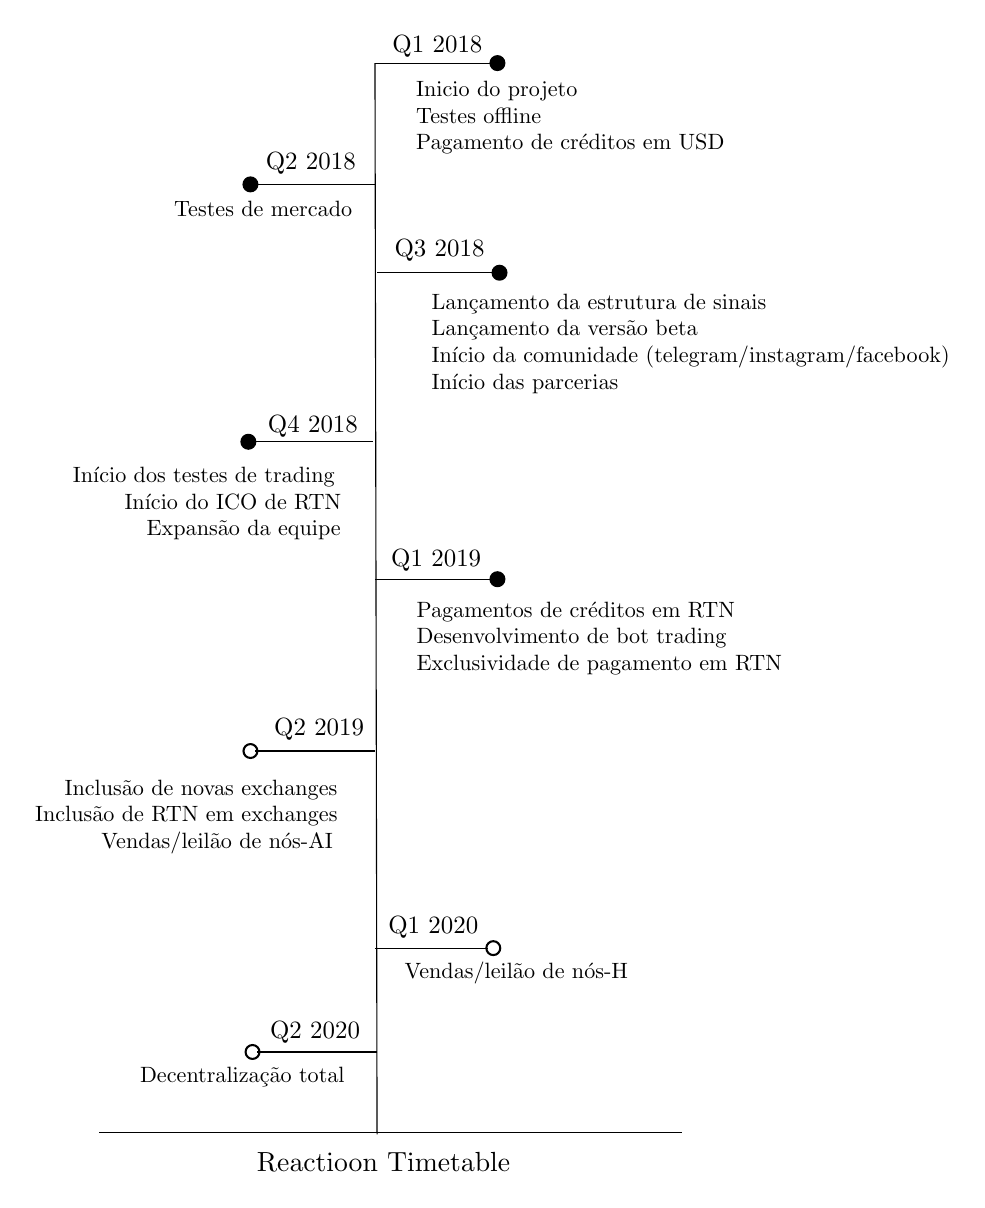
\begin{tikzpicture}[x=0.75pt,y=0.75pt,yscale=-1,xscale=1]
%uncomment if require: \path (0,600.9199981689453); %set diagram left start at 0, and has height of 600.9199981689453

%Straight Lines [id:da27949880366729407] 
\draw    (290.9,47.8) -- (291.9,563.92) ;


%Straight Lines [id:da016695516966388713] 
\draw    (290.9,47.8) -- (349.9,47.8) ;
\draw [shift={(349.9,47.8)}, rotate = 0] [color={rgb, 255:red, 0; green, 0; blue, 0 }  ][fill={rgb, 255:red, 0; green, 0; blue, 0 }  ][line width=0.75]      (0, 0) circle [x radius= 3.35, y radius= 3.35]   ;

%Straight Lines [id:da04938623797133035] 
\draw    (290.9,106.24) -- (230.9,106.24) ;
\draw [shift={(230.9,106.24)}, rotate = 180] [color={rgb, 255:red, 0; green, 0; blue, 0 }  ][fill={rgb, 255:red, 0; green, 0; blue, 0 }  ][line width=0.75]      (0, 0) circle [x radius= 3.35, y radius= 3.35]   ;

%Straight Lines [id:da10792958400592911] 
\draw    (290.9,379.24) -- (233.25,379.24) ;
\draw [shift={(230.9,379.24)}, rotate = 180] [color={rgb, 255:red, 0; green, 0; blue, 0 }  ][line width=0.75]      (0, 0) circle [x radius= 3.35, y radius= 3.35]   ;

%Straight Lines [id:da5389580478447318] 
\draw    (289.9,230.24) -- (229.9,230.24) ;
\draw [shift={(229.9,230.24)}, rotate = 180] [color={rgb, 255:red, 0; green, 0; blue, 0 }  ][fill={rgb, 255:red, 0; green, 0; blue, 0 }  ][line width=0.75]      (0, 0) circle [x radius= 3.35, y radius= 3.35]   ;

%Straight Lines [id:da7641576297357624] 
\draw    (291.9,148.8) -- (350.9,148.8) ;
\draw [shift={(350.9,148.8)}, rotate = 0] [color={rgb, 255:red, 0; green, 0; blue, 0 }  ][fill={rgb, 255:red, 0; green, 0; blue, 0 }  ][line width=0.75]      (0, 0) circle [x radius= 3.35, y radius= 3.35]   ;

%Straight Lines [id:da04724001416544876] 
\draw    (290.9,296.46) -- (349.9,296.46) ;
\draw [shift={(349.9,296.46)}, rotate = 0] [color={rgb, 255:red, 0; green, 0; blue, 0 }  ][fill={rgb, 255:red, 0; green, 0; blue, 0 }  ][line width=0.75]      (0, 0) circle [x radius= 3.35, y radius= 3.35]   ;

%Straight Lines [id:da9347215346833444] 
\draw    (290.9,474.2) -- (345.55,474.2) ;
\draw [shift={(347.9,474.2)}, rotate = 0] [color={rgb, 255:red, 0; green, 0; blue, 0 }  ][line width=0.75]      (0, 0) circle [x radius= 3.35, y radius= 3.35]   ;

%Straight Lines [id:da28779960793088244] 
\draw    (291.9,524.24) -- (234.25,524.24) ;
\draw [shift={(231.9,524.24)}, rotate = 180] [color={rgb, 255:red, 0; green, 0; blue, 0 }  ][line width=0.75]      (0, 0) circle [x radius= 3.35, y radius= 3.35]   ;

%Straight Lines [id:da8846097036360219] 
\draw    (158,563) -- (438.9,563) ;



% Text Node
\draw (385,74.02) node [scale=0.8] [align=left] {Inicio do projeto\\Testes offline\\Pagamento de créditos em USD};
% Text Node
\draw (290,55) node [scale=0.8] [align=left] {};
% Text Node
\draw (237,118) node [scale=0.8] [align=left] {Testes de mercado};
% Text Node
\draw (443,183) node [scale=0.8] [align=left] {Lançamento da estrutura de sinais\\Lançamento da versão beta\\Início da comunidade (telegram/instagram/facebook)\\Início das parcerias};
% Text Node
\draw (321,40) node [scale=0.9] [align=left] {Q1 2018};
% Text Node
\draw (260,96) node [scale=0.9] [align=left] {Q2 2018};
% Text Node
\draw (322,138) node [scale=0.9] [align=left] {Q3 2018};
% Text Node
\draw (261,223) node [scale=0.9] [align=left] {Q4 2018};
% Text Node
\draw (320.4,287.46) node [scale=0.9] [align=left] {Q1 2019};
% Text Node
\draw (264,369) node [scale=0.9] [align=left] {Q2 2019};
% Text Node
\draw (319,464.16) node [scale=0.9] [align=left] {Q1 2020};
% Text Node
\draw (262,515) node [scale=0.9] [align=left] {Q2 2020};
% Text Node
\draw (321,158) node [scale=0.8] [align=left] {};
% Text Node
\draw (210,260) node [scale=0.8] [align=left] {Início dos testes de trading\\ \ \ \ \ \ \ \ Início do ICO de RTN\\ \ \ \ \ \ \ \ \ \ \ Expansão da equipe};
% Text Node
\draw (399,325) node [scale=0.8] [align=left] {Pagamentos de créditos em RTN\\Desenvolvimento de bot trading\\Exclusividade de pagamento em RTN};
% Text Node
\draw (200,411) node [scale=0.8] [align=left] { \ \ \ \ Inclusão de novas exchanges\\Inclusão de RTN em exchanges\\ \ \ \ \ \ \ \ \ \   Vendas/leilão de nós-AI};
% Text Node
\draw (359,486) node [scale=0.8] [align=left] {Vendas/leilão de nós-H};
% Text Node
\draw (227,536) node [scale=0.8] [align=left] {Decentralização total};
% Text Node
\draw (295,577) node  [align=left] {Reactioon Timetable};


\end{tikzpicture}
}
\caption{Timetable diagram}
\end{figure}
\section{RTN token}
The RTN token may be used within the Reactioon ecosystem and will be traded at the exchanges where it will be listed. We understand that the value of the token will be proportional to the profits that robots will return to the investors.

1 RTN corresponds to 1 credit available on the trading platform. Currently each credit allow users to use the robot for 1-day period. Subsequently it is intended to define operating volume ranges so that the credits charged are proportional to the profit volumes.

\subsection{ICO}
Our ICO will be released on 09-09-2018 and will last until the end of the available tokens. The prices of each token will be initially set at USD 1. However, the firsts adepts of our platform will get a progressive discount as described bellow:

\begin{table}[!h]
        \centering
        
\begin{tabular}{p{0.2\textwidth}p{0.2\textwidth}|p{0.2\textwidth}}
\begin{center}
\textbf{From}
\end{center}
 & \begin{center}
\textbf{To}
\end{center}
 & \begin{center}
\textbf{ICO token price}
\end{center}
 \\
\hline 
 \begin{center}
{\small 0}
\end{center}
 & \begin{center}
{\small 100,000}
\end{center}
 & \begin{center}
{\small USD 0.25}
\end{center}
 \\
\hline 
 \begin{center}
{\small 100,000}
\end{center}
 & \begin{center}
{\small 500,000}
\end{center}
 & \begin{center}
{\small USD 0.50}
\end{center}
 \\
\hline 
 \begin{center}
{\small 500,000}
\end{center}
 & \begin{center}
{\small 1,000,000}
\end{center}
 & \begin{center}
{\small USD 0.75}
\end{center}
 \\
\hline 
 \begin{center}
{\small 1,000,000}
\end{center}
 & \begin{center}
{\small 3,000,000}
\end{center}
 & \begin{center}
{\small USD 1.00}
\end{center}
 \\

\end{tabular}
        \end{table}


\subsection{Airdrops}
RTN airdrops will be available during each new listing on a new exchange.

\subsubsection{Token division}
\begin{itemize}
    \item [] Founders: 3,000,000
    
    \item [] ICO: 3,000,000

    \item [] Cold Wallet: 15,000,000

    \item [] Total supply: 21,000,0000

\end{itemize}

\section{Conclusion}

We at Reactioon intend to change the way asset management is performed in the world. We understand that our model is comparable to that of an investment bank, but differently from them, we are totally transparent and our managers are a group of artificial intelligence machines and humans-aided by machines.

If you do share our philosophy ans belive in the future of crypto-assets, we at Reactioon invite you to our community and to share our business. We're just starting a big change! Join us. 


Reactioon: The future is now!

% Tabelas devem ser centradas na página e numeradas com algarismos arábicos.  A legenda deve ficar acima da tabela.   Linhas verticais são opcionais.  Separe a figura do texto anterior com um espaço de 12 pt. 

%\section{Equações}

%Equações devem separadas do texto por espaços de 6 pt (meia linha) antes e depois.  Numere as equações com algarismos arábicos, colocados entre parênteses e alinhados à esquerda,  como mostra o exemplo a seguir.

%\begin{equation}
%x = y+1.
%\end{equation}

%Pontue a equação e continue o texto seguinte como se a equação fosse parte do texto.  Por exemplo, a equação 1 termina com um ponto final e o parágrafo seguinte a ela (que é este) começa em maiúscula e com tabulação.  Segundo exemplo: em

%\begin{displaymath}
%y = x-1,
%\end{displaymath}

%segue-se a equação 2 com uma vírgula, e o parágrafo seguinte (que é este) começa em minúscula e sem tabulação. Utilize "\$"  para inserir equações no meio do texto, como em $y=x-2$.

%\section{Referências Bibliográficas}

%Referências devem ser citadas no texto no formato (SOBRENOME, ano) ou (SOBRENOME1 e SOBRENOME2, ano), entre parênteses, com os sobrenomes dos autores em maiúscula e o ano de publicação com 4 dígitos.  Havendo muitos autores, indique o primeiro e abrevie os demais com “et al.” – por exemplo (FULANO et al., 1998).

%Caso deseje citar uma obra forma textual no artigo, inclua o ano da publicação entre parênteses após o(s) nome(s) dos autor(es).  Por exemplo: “Segundo Fulano e Sicrano (1999), é possível que...”.

%Para mais informações sobre como citar adequadamente diferentes tipos de trabalho, consulte por exemplo as diretrizes compiladas pela Divisão de Bibliotecas da Escola Politécnica da USP (2013), disponível em

%http://www.poli.usp.br/images/stories/media/download/bibliotecas/DiretrizesTesesDissertacoes.pdf

%\appendix
%\section*{Apêndices}
 
%A seção de apêndices é opcional.  Se precisar incluí-la, deixe 24 pt (duas linhas) de espaço antes do título “Apêndices”,  escrito centrado na linha, em letras maiúsculas (ou versalete) e tamanho 14 pt.
 
%\addcontentsline{toc}{section}{Apêndices}   % Definindo seção de apêndice
%\renewcommand{\thesection}{\textit{\Alph{section}} }
%\section{\textit{Primeiro apêndice}}
 
%Deixe um espaço de 12 pt antes e depois do título do apêndice.  Escreva o título em tamanho 14 pt e em itálico.  Os apêndices devem ser numerados com letras maiúsculas.


%\section*{Agradecimentos}

%Agradecimentos (opcional).  Deixe um espaço de 24 pt antes do título “Agradecimentos”, escrito centrado na linha, em maiúscula (ou versalete) e tamanho 14 pt.  Escreva o texto dos agradecimentos após um espaço de 12 pt.

% \centering\section*{REFERENCES}
%O título da seção de referências deve ter um espaço antes de 24 pt e deve ser escrito centrado na linha, em maiúscula (ou versalete) e tamanho 14 pt.  Deixe um espaço de 12 pt antes do texto da primeira referência.  Deixe um espaço de 6 pt (meia linha) entre as referências.

%Liste as obras pela ordem alfabética do sobrenome do primeiro autor (ou nome da empresa).  Não numere as referências.  Alguns exemplos:

%\noindent SOBRENOME, Nome. Título da publicação.  Edição, Cidade de publicação: Editora, ano, páginas $\{ $Referencia$\} $.

%\noindent SOBRENOME1, Nome1;  SOBRENOME2, Nome2.  Título da publicação.  Edição, Cidade de publicação: Editora, ano, páginas.

%\noindent SOBRENOME1, Nome1;  SOBRENOME2, Nome2; et al.  Título da publicação.  Edição, Cidade de publicação: Editora, ano, páginas.

%Também é possível utilizar o comando \textbackslash bibliography\{\} do LaTeX para inserir as referências a partir de um arquivo .bib, como mostrado a seguir. Para as referências presentes no arquivo .bib aparecerem nessa seção, elas devem ter sido citadas em algum ponto do artigo com o comando \textbackslash cite\{\}, como a seguir: \cite{referencia1}, \cite{referencia2} e \cite{referencia3}.

%\vspace{-8mm}
\begingroup
\makeatletter
\renewcommand{\chapter}{\@gobbletwo}
\makeatother
\bibliographystyle{abntex2-alf-mod}
\bibliography{mybibfile}
\endgroup

%(Se seu artigo não for escrito em inglês, acrescente aqui as versões em inglês do título, resumo e palavras-chaves)

%\begin{changemargin}{1cm}{1cm} 

%Title: Template for Papers of the Mecatrone Journal 

%\textbf{Abstract} – This is the English version of the resume.

%\textbf{Keywords} – Comma separated list of keywords.

%\end{changemargin}

% \begin{figure}[h]
%     \includegraphics[width=0.5\textwidth]{figure2}
%     \caption{figura2}
%     \label{figura2}
% \end{figure}

\textbf{José Wilker}, Creator of Reactioon technology. Full stack specialist. expert in PHP / Javascript / NodeJS / C / ShellScript , with background in agile techniques for Project Management and Linux. Loves Math, Chess, Cards and RPG/Strategy Games.

\textbf{Jonathas Marcelo Pereira Figueiredo}, Graduated in Mechatronics Engineering at Escola Politécnica of the University of São Paulo, Brazil. Graduated in Automated Systems and  Information Engineering at ENSE3 Grenoble-INP, France.

\textbf{Lucas Tonini}, Marketing specialist with experience in digital campaigns advisory.


% \begin{figure}[h]
%     \includegraphics[width=0.5\textwidth]{figure2}
%     \caption{figura2}
%     \label{figura2}
% \end{figure}



\end{document}